\section{Verifying a Realistic Context Switch Module}
\label{sec:ctxswitch}

\indent
We apply our program logic to verify
the main body of a context switch routine implemented in \sparc,
which is used to save the current task's context and
restore the new task's context.
\Fig{\ref{fig:The Structure of Context Switch Module}}
shows the structure of the code.
%And we describe the function of a part of them informally.

\begin{center}
    \vspace*{-1.5em}
	\centering
	%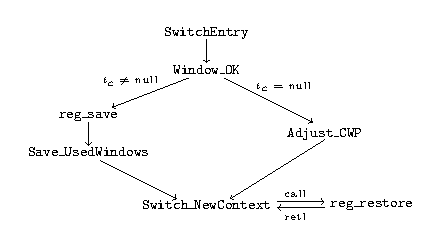
\includegraphics[scale=1.3]{picture//CodeStructure}
	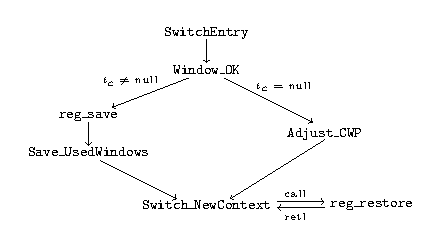
\includegraphics[scale=1.1]{picture//CodeStructure}
	\vspace{-0.4cm}
    \figurecaption{The Structure of Context Switch Module}
	\label{fig:The Structure of Context Switch Module}
\end{center}

% \begin{figure}[!t]
% 	\vspace{-0.8cm}
% 	\centering
% 	%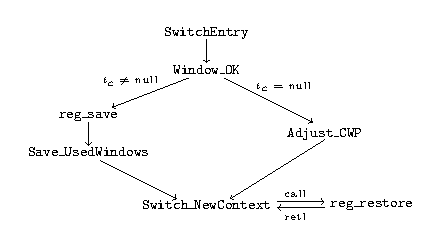
\includegraphics[scale=1.3]{picture//CodeStructure}
% 	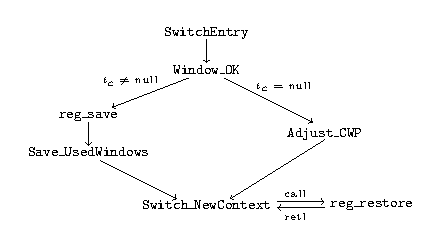
\includegraphics[scale=1.2]{picture//CodeStructure}
% 	\vspace{-0.4cm}
%     \caption{The Structure of Context Switch Module}
% 	\label{fig:The Structure of Context Switch Module}
% 	\vspace{-0.2cm}
% \end{figure}

\begin{itemize}
	\item
	\texttt{SwitchEntry}
    is the entry of the module.
	It checks {\tt SwitchFlag} to see if
    a context switch is needed. If yes,
    it enters the $\texttt{Window\_OK}$ block.
	
	\item
	\texttt{Window\_OK}
    checks if the current task is null (which may happen
    if the switch follows the delete of the current task).
    If yes, it jumps to \texttt{Adjust\_CWP}, which
    resets the pointer $\regcwp$ of the current register window
    so that it points to the last valid window. It essentially pops
    all the frames to empty the circular stack of register
    windows.
    If the current task is {\em not} null,
    it calls \texttt{reg\_save} to save the
    general registers into the TCB, and then
    enter the code block \texttt{Save\_UsedWindows}
    to save other register windows ($\Wstack$ in our
    state model).
	
	\item
	\texttt{Save\_UsedWindows} saves
	the register windows (except the current one)
    into the current task's stack in memory. 
    It checks whether the previous window is valid. 
    If it's valid, use the instruction $\crestore{}$ 
    to set the previous window as the current one, 
    and save its contents into stack (in memory), 
    then check the previous one continuously. 
	
	\item
	\texttt{Switch\_NewContext}
    %is responsible for
%	restoring the context stored in new task's TCB
%	and the other context saved in the top of the new task's stack.
%	Then it changes the new task as the current.
    restores the general registers and other register
    windows from the new task's TCB and its stack in memory,
    respectively. Then it sets the new task as
    the current one.
%    the new task's context from its TCB
%    and its stack in memory.
%    Then it changes the new task as the current one.
%>>>>>>> .r75
\end{itemize}

%\paragraph{\bf Challenge.}
The main complexity of the verification lies in
the code manages the register windows.
%The major difference between the context switch module we verified
%and a traditional one is caused by the register windows mechanism in \sparc{}.
%We have introduced that the register windows play as a role of circular stack.
%However, a stack in memory is still needed here because the number of windows is limited.
%
To save all the register windows, \texttt{Save\_UsedWindows}
repetitively restores the next window into general registers
(as the current window)
and then saves them into memory, until all the windows are saved.

%The code block \texttt{Save\_UsedWindows} is responsible
%for saving the contexts stored in register windows temporarily
%into current task's stack in memory when doing context switch.
%It restores the next window by window rotation and saves its contents into memory repeatedly,
%until the next window is an invalid one, which can be viewed a stack bottom.
%So, the implementation of \texttt{Save\_UsedWindows} is a loop
%and its verification work requires us to take more effort.

\paragraph{\textbf{Specification.}}
Below we give the pre- and post-conditions
($\apre$ and $\apost$) of the verified module.
Each of them takes 5 arguments,
the id of the current task $\ctid$, the id of the new
task $\ntid$, the value $\flag$ of the $\SwitchFlag$,
the values $\env$ of general registers and all
other register windows, and the new task's context $\nst$
that needs to be restored.
\[
    \small
    \begin{array}{l}
        \apre(\ctid, \ntid, \flag, \env, \nst) \ \define \\
        \qquad
        \begin{array}{l}
            \Env{\env} \sepstar (\msto{\SwitchFlag}{\flag}) \sepstar (\msto{\TaskNew}{\ntid})
            \sepstar \\
            \hspace*{8ex}
            (\flag\! =\! \afalse
            \vee \CurTask{\ctid}{\notCare}{\env}
                \!*\! \NoCurTask{\ntid}{\nst})
        \end{array}
        \\
        \\[-9pt]
        \apost(\ctid, \ntid, \flag, \env, \nst) \ \define \\
        \qquad
        \begin{array}{l}
            \Env{\env'} \sepstar (\msto{\SwitchFlag}{\afalse})
                    \sepstar (\msto{\TaskNew}{\ntid}) \sepstar
            \\
            \hspace*{8ex}
            (
            \flag \!=\! \afalse \land \pEnv{\env} \!=\! \pEnv{\env'}
            \\
            \quad \hspace*{8ex}
            \vee (\CurTask{\ntid}{\nst}{\env'} \land \pEnv{\env'}\!=\!\nst) *
            \\
            \quad \hspace*{12ex}
            \NoCurTask{\ctid}{\pEnv{\env}})        
        \end{array}
    \end{array}
    % \begin{array}{lcl}
    %     \apre(\ctid, \ntid, \flag, \env, \nst) & \define &
    %     \Env{\env} * (\msto{\SwitchFlag}{\flag}) * (\msto{\TaskNew}{\ntid}) * \\
    %     & & \hspace*{8ex}
    %     (\flag\! =\! \afalse
    %     \vee \CurTask{\ctid}{\notCare}{\env}
    %             \!*\! \NoCurTask{\ntid}{\nst}) \\
    %     %
    %     \apost(\ctid, \ntid, \flag, \env, \nst) & \define & \exists \env{}'. \
    %     \Env{\env'} * (\msto{\SwitchFlag}{\afalse})
    %                 * (\msto{\TaskNew}{\ntid}) *
    %     \\
    %     & & \hspace*{8ex}
    %     (
    %         \flag \!=\! \afalse \land \pEnv{\env} \!=\! \pEnv{\env'}
    %         \\
    %         & & \quad \hspace*{8ex}
    %         \vee (\CurTask{\ntid}{\nst}{\env'} \land \pEnv{\env'}\!=\!\nst) *
    %         \\
    %         & & \quad \hspace*{12ex}
    %         \NoCurTask{\ctid}{\pEnv{\env}})
    % \end{array}
\]

%specification of the key component of the context switch module verified,
%which is used to saving the current task's context and restore a new one.
%Five parameters are needed for specification that
%(1) $\ctid$ is the current task's identifier,
%(2) $\ntid$ is the new task's identifier,
%(3) $\flag$ presents the value of $\SwitchFlag$ which marks
%    whether there is a requirement to switch to a new task,
%(4) $\env$ presents the values stored in general registers and register windows,
%and
%(5) $\nst$ is the context of new task that will be restored.

In the specification,
we use $\Env{\env}$ to specify the values of
general registers and the register windows.
The variable $\TaskNew$ records the identifier of the new task.
If $\SwitchFlag$ is $\afalse$, we do not need any knowledge
about the current and the new tasks since there is no
context switch. Otherwise we describe the state
of the current task (its TCB and stack in memory)
using $\CurTask{\ctid}{\notCare}{\env}$,
and the saved context of the new task using
$\NoCurTask{\ntid}{\nst}$.
Due to space limitation we omit the detailed
definitions here.

If we compare $\apre$ and $\apost$, we can see that
$\ntid$ becomes the current task
($\CurTask{\ntid}{\nst}{\env'}$),
and its general registers and stack, specified by
$\Env{\env'}$, are loaded from the saved context
$\nst$ (\ie{} $\pEnv{\env'}\!=\!\nst$).
%$(\CurTask{\ntid}{\nst}{\env'} \land \pEnv{\env'}\!=\!\nst)$.
Here $\pEnv{\env'}$ refers to the part of the environment
that we want to save or restore as context.
Correspondingly, $\ctid$ becomes non-current-thread,
and part of its environment $\env$ at the entry of
the context switch is saved, as specified
by $\NoCurTask{\ctid}{\pEnv{\env}}$.

%\indent
%The precondition $\apre$ is shown below.
%The $\Env{\env}$ is used to describe the state of
%general registers and the register windows
%and uses $\env$ as parameter.
%The variable $\TaskNew$ records the identifier of the new task.
%We can see that if the value of the $\SwitchFlag$ is $\afalse$,
%we don't have to know anything about current task and new task,
%because there is no requirement to do context switch and
%the program exits directly.
%We describe the state of current task by $\CurTask{\ctid}{\notCare}{\env}$
%and the new task by $\NoCurTask{\ntid}{\nst}$.
%\[
%    \small
%    \begin{array}{lcl}
%        \apre(\ctid, \ntid, \flag, \env, \nst) & \define &
%        \Env{\env} * \msto{\SwitchFlag}{\flag} * \msto{\TaskNew}{\ntid} \\
%        & & \hspace*{12ex} * (\flag = \afalse \vee (\CurTask{\ctid}{\notCare}{\env} * \NoCurTask{\ntid}{\nst})) \\
%    \end{array}
%\]
%
%\indent
%We define the postcondition as $\apost$.
%It tells us that the new task $\ntid$ will become the
%current task and
%original current one will be the non-current task,
%if the $\flag$ is $\atrue$.
%Here, the $\pEnv{\env}$ is used to extract part
%of dates that the task hopes to save.
%%\[
%%    \small
%%    \begin{array}{lcl}
%%        \apost(\ctid, \ntid, \flag) & \define &
%%        \exists \env, \cst, \nst. \\
%%        & & \ \
%%        \Env{\env} * \msto{\SwitchFlag}{\afalse} * \msto{\TaskNew}{\ntid} \\
%%        & & \ \
%%        * (\flag = \afalse \, \vee \,
%%            (\flag = \atrue \, \land \, (\CurTask{\ntid}{\nst}{\env} * \NoCurTask{\ctid}{\cst}))
%%        )
%%    \end{array}
%%\]
%\[
%    \small
%    \begin{array}{lcl}
%        \apost(\ctid, \ntid, \flag, \env, \nst) & \define & \exists \env{}'. \
%        \Env{\env'} * \msto{\SwitchFlag}{\afalse} * \msto{\TaskNew}{\ntid} \\
%        & & *
%        (
%            (\flag = \afalse \land \pEnv{\env} = \pEnv{\env'}) \\
%            & & \quad \vee (\CurTask{\ntid}{\nst}{\env'} * \NoCurTask{\ctid}{\pEnv{\env}}))
%    \end{array}
%\]
%

%\indent
%The $\NoCurTask{\tid}{\tskst}$ describes the state of task $\tid$'s
%context structure and stack in memory, if $\tid$ is not \Null{}. The context structure,
%which is a part of TCB  for registers data saving, is presented as
%$\context{\tid + \offsetctx, \ctx}$, where its address is $\tid + \offsetctx$.
%And $\stackCons{\stk}$ presents the state of task's stack in memory.
%Here $\Top$ is the address of stack top and $\stkcont$ is the values
%saved in stack.
%The $\stkfmPt{\Top}{\env}$ used in $\CurTask{\tid}{\tskst}{\env}$
%illustrates a pointing relationship between register windows and task's stack.
%It says that each context saved in register windows temporarily records a pointer that points to
%a stack frame in stack where it will be stored.
%\[
%    \small
%    \begin{array}{lcl}
%        \NoCurTask{\tid}{\tskst} & \define &
%        (\tid \neq \Null \, \land \, (\context{\tid + \offsetctx, \ctx} * \stackCons{\stk}))
%        \, \vee \, \tid = \Null
%        \\
%        & & \ \ {\text{where} \ \tskst = (\ctx, \stk), \, \stk = (\Top, \stkcont)} \\
%        \\[-8pt]
%        \CurTask{\tid}{\tskst}{\env} & \define &
%        (\msto{\TaskCur}{\tid} * \NoCurTask{\tid}{\tskst}) \, \land \,
%        \stkfmPt{\Top}{\env} \\
%        & & \ \ {\text{where} \ \tskst = (\ctx, \stk), \, \stk = (\Top, \stkcont)}
%    \end{array}
%\]
\begin{figure*}[!t]
    \[
        \begin{array}{c}
            \infer[L_3]
            {
                (\regst{\regN}{\val}) \sepstar \astP_1 \Longrightarrow 
                (\regst{\regN}{\val}) \sepstar \astP_2
            }
            {
                \astP_1 \Longrightarrow \astP_2
            } \qquad 
            \infer[L_4]
            {
                (\dlyregst{t}{\st}{\word}) \sepstar \astP_1 \Longrightarrow 
                (\dlyregst{t}{\st}{\word}) \sepstar \astP_2
            }
            {
                \astP_1 \Longrightarrow \astP_2
            } \\
            \\[-5pt]
            \infer[L_3]
            {
                \nxtAst{(\dlyregst{0}{\sr}{\word})} \sepstar \astP_2 \Longrightarrow 
                (\regst{\sr}{\word}) \sepstar \astP_2
            }
            {
                \astP_1 \Longrightarrow \astP_2
            } \quad \ \ 
            \infer[L_4]
            {
                \nxtAst{(\dlyregst{t+1}{\sr}{\word})} \sepstar \astP_1 \Longrightarrow 
                (\dlyregst{t}{\sr}{\word}) \sepstar \astP_2
            }
            {
                \astP_1 \Longrightarrow \astP_2
            } \\
            \\[-5pt]
            \infer[L_5]
            {
                \nxtAst{(\regst{\regN}{\val})} \sepstar \astP_1 \Longrightarrow 
                \regst{\regN}{\val} \sepstar \astP_2
            }
            {
                \astP_1 \Longrightarrow \astP_2
            } \qquad 
            \infer[L_6]
            {
                \nxtAst{(\sepsto{\loc}{\val})} \sepstar \astP \Longrightarrow 
                (\sepsto{\loc}{\val}) \sepstar \astP'
            }
            {
                \astP_1 \Longrightarrow \astP_2
            } \quad \ \
            \infer[L_7]
            {
                \nxtAst{(\astP_1 \sepstar \astP_2)}
                \Longrightarrow 
                \astP_1' \sepstar \astP_2'
            }
            {
                \nxtAst{\astP_1} \Longrightarrow \astP_1' \quad \ \ 
                \nxtAst{\astP_2} \Longrightarrow \astP_2'
            } 
        \end{array}
    \]
    \caption{Extended rules for Tactic \sepcancel{}}
    \label{fig:ext-rule-tac-sepcancel}
\end{figure*}
\paragraph{\textbf{Tactics for Automated Reasoning.}} 
\etal{Cao}\cite{practical-tactics} propose a set of practical tactics 
for verifiying C program in Coq. 
including \sepcancel{}, which uses some 
inference rules (\eg{} $L_1$ and $L_2$ shown as following) 
repeatedly to solve $\astP \Longrightarrow \astQ$. 
\[
    \small
    \infer[L_1]
    {
        \astP_1 \sepstar \astQ' \Longrightarrow \astP_2 \sepstar \astQ'
    }
    {
        \astP_1 \Longrightarrow \astP_2
    } \quad \ \  
    \infer[L_2]
    {
        (\sepsto{\loc}{\val}) \sepstar \astP_1 \Longrightarrow 
        (\sepsto{\loc}{\val}) \sepstar \astP_2
    }
    {
        \astP_1 \Longrightarrow \astP_2
    }
\]
One of a important tacitc in their work is \sepcancel{}. 
It has a library, including some rules (\eg{} $L_1$ and $L_2$ shown above), 
and uses the rules in library repeatedly to solve 
``$\astP \Longrightarrow \astQ$". The rules $L_1$ and $L_2$  
let we can use \sepcancel{} to eliminate the 
subterms, which describe the same resources, 
in $\astP$ and $\astQ$.
Recalling the introduction in \Sec{\ref{subsec:assertions}}, 
registers in our work are also treated as resource. 
So, we extend the inference rules used by original \sepcancel{} tactics
and let it  

Recalling the introduction in \Sec{\ref{subsec:assertions}}, 
registers in our work are also treated as resource, like memory location. 
In our work, we add some additional rules $L_3 \sim L_7$ 
(defined in \Fig{\ref{fig:ext-rule-tac-sepcancel}})
to the library of \sepcancel{}. The soundness of rules $L_3 \sim L_7$ 
can be achieved from the properties of assertions introduced in 
\Sec{\ref{subsec:assertions}} directly. Aftering extending the original 
\sepcancel{} tactic, we can find that the correctness proof
of the following implication can be accomplished by using 
the extended \sepcancel{} directly.
\begin{multline*}
    \nxtAst{(\dlyregst{3}{\regY}{\word_1} \sepstar 
    \dlyregst{0}{\regwim}{\word_2} \sepstar 
    \regst{\reg{5}}{\val})} \Longrightarrow \\
    \dlyregst{2}{\regY}{\word_1} \sepstar 
    \regst{\regwim}{\word_2} \sepstar 
    \regst{\reg{5}}{\val}
\end{multline*}
\[
    \nxtAst{(\dlyregst{3}{\regY}{\word_1} \sepstar 
    \dlyregst{0}{\regwim}{\word_2} \sepstar 
    \regst{\reg{5}}{\word_3})} \Longrightarrow 
    \dlyregst{2}{\regY}{\word_1} \sepstar 
    \regst{\regwim}{\word_2} \sepstar 
    \regst{\reg{5}}{\word_3}
\] 
Using the extended \sepcancel{} can greatly simplify our verification 
work, and improve the efficiency of code proving. 

\paragraph{\textbf{Proof Efforts in Coq.}}
We omit the code that manages interrupt
and float registers in the original
system, which are not supported in our logic.
%because our current work doesn't consider them.
The segment we verify has around 250 lines
of assembly code,
and we verify it by 6690 lines of %(including the tactics and libraries)
Coq proof scripts.

% We briefly show how we verify the 
% context switch routine in Coq using our program logic. 
% % % \begin{figure}[!t]
%     \centering
%     \small
%     \[
%         \begin{array}{c|c}
%         \begin{array}{l}
%             {\tt Theorem \ \ CtxSwitch\_Correct: } \\
%             \qquad 
%             {\tt wf\_cdhp \ \, spec \ C}. \\
%             {\tt Proof. }  \\
%             \qquad \dots \ \ \dots \ \ \dots \\ 
%             {\tt Qed. }
%         \end{array} \quad & \quad
%         \begin{array}{l}
%             {\tt Lemma \ \ SwitchEntryProof: } \\
%             \qquad 
%             {\tt forall \ vl,} \\
%             \qquad \qquad
%             {\tt spec \ |- \ \{\{ \ \colorbox{yellow!80}{switch\_entry\_pre \ vl} \ \}\} } \\
%             \qquad \qquad \qquad \qquad \qquad
%             {\tt f0 : switch\_entry\_code} \\
%             \qquad \qquad \qquad \qquad
%             {\tt \ \{\{ \ \colorbox{yellow!80}{switch\_entry\_post \ vl} \ \}\}. } \\
%             {\tt Proof.} \\
%             \qquad \dots \ \ \dots \ \ \dots \\ 
%             {\tt Qed. }
%         \end{array} \\
%         \\[-5pt]
%         \text{(a)} & \text{(b)}
%         \end{array}
%     \]
%     \caption{Example of Context Switch Routine Proof in Coq}
%     \label{fig:CorrectCtx-Coq}
%     \vspace{-0.5em}
% \end{figure}

\begin{figure}[!t]
    \centering
    \small
    \[
        \begin{array}{c|c}
        \begin{array}{l}
            {\tt Theorem \ \ CtxSwitch\_Correct: } \\
            \qquad 
            {\tt wf\_cdhp \ \, spec \ C}. \\
            {\tt Proof. }  \\
            \qquad \dots \ \ \dots \ \ \dots \\ 
            {\tt Qed. }
        \end{array} \quad & \quad
        \begin{array}{l}
            {\tt Lemma \ \ SwitchEntryProof: } \\
            \qquad 
            {\tt forall \ vl,} \\
            \qquad \qquad
            {\tt spec \ |- \ \{\{ \ \colorbox{yellow!80}{switch\_entry\_pre \ vl} \ \}\} } \\
            \qquad \qquad \qquad \qquad \qquad
            {\tt f0 : switch\_entry\_code} \\
            \qquad \qquad \qquad \qquad
            {\tt \ \{\{ \ \colorbox{yellow!80}{switch\_entry\_post \ vl} \ \}\}. } \\
            {\tt Proof.} \\
            \qquad \dots \ \ \dots \ \ \dots \\ 
            {\tt Qed. }
        \end{array} \\
        \\[-5pt]
        \text{(a)} & \text{(b)}
        \end{array}
    \]
    \caption{Example of Context Switch Routine Proof in Coq}
    \label{fig:CorrectCtx-Coq}
    \vspace{-0.5em}
\end{figure}
% \begin{center}
%     \vspace*{-0.8cm}
%     $$ \ 
%     {\tt Theorem \ \ CtxSwitch\_Correct: } \ \ 
%     {\tt wf\_cdhp \ \, spec \ C}.
%     $$
%     $$
%     \begin{array}{l}
%         {\tt Lemma \ \ SwitchEntryProof: } \\
%         \qquad 
%         {\tt forall \ vl,} \\
%         \qquad \qquad
%         {\tt spec \ |- \ \{\{ \ \colorbox{yellow!80}{switch\_entry\_pre \ vl} \ \}\} } \\
%         \qquad \qquad \qquad \qquad \qquad
%         {\tt f0 : switch\_entry\_code} \\
%         \qquad \qquad \qquad \qquad
%         {\tt \ \{\{ \ \colorbox{yellow!80}{switch\_entry\_post \ vl} \ \}\}. }
%     \end{array}
%     $$
%     \figurecaption{Coq Code Example}
%     \label{fig:Coq code Example}
% \end{center}
% % \begin{figure}[!t]
% %     \centering
% %     \small
% %     \[
% %         \begin{array}{c|c}
% %         \begin{array}{l}
% %             {\tt Theorem \ \ CtxSwitch\_Correct: } \\
% %             \qquad 
% %             {\tt wf\_cdhp \ \, spec \ C}. \\
% %             {\tt Proof. }  \\
% %             \qquad \dots \ \ \dots \ \ \dots \\ 
% %             {\tt Qed. }
% %         \end{array} \quad & \quad
% %         \begin{array}{l}
% %             {\tt Lemma \ \ SwitchEntryProof: } \\
% %             \qquad 
% %             {\tt forall \ vl,} \\
% %             \qquad \qquad
% %             {\tt spec \ |- \ \{\{ \ \colorbox{yellow!80}{switch\_entry\_pre \ vl} \ \}\} } \\
% %             \qquad \qquad \qquad \qquad \qquad
% %             {\tt f0 : switch\_entry\_code} \\
% %             \qquad \qquad \qquad \qquad
% %             {\tt \ \{\{ \ \colorbox{yellow!80}{switch\_entry\_post \ vl} \ \}\}. } \\
% %             {\tt Proof.} \\
% %             \qquad \dots \ \ \dots \ \ \dots \\ 
% %             {\tt Qed. }
% %         \end{array} \\
% %         \\[-5pt]
% %         \text{(a)} & \text{(b)}
% %         \end{array}
% %     \]
% %     \caption{Example of Context Switch Routine Proof in Coq}
% %     \label{fig:CorrectCtx-Coq}
% %     \vspace{-0.5em}
% % \end{figure}
% The Coq theorem named ``{\tt CtxSwitch\_Correct}" in 
% \Fig{\ref{fig:Coq code Example}} is the final theorem of 
% the correctness of context routine in Coq.
% % \Fig{\ref{fig:CorrectCtx-Coq}} (a) is the final theorem of 
% % the correctness of context routine in Coq. The 
% % ``{\tt CtxSwitch\_Correct}" is the name of this 
% % theorem. And 
% The ``{\tt wf\_cdhp spec C}" is the  
% Coq implementation of well-formed code heap 
% ``$\wfcdhp{\code}{\Cspec}$". Here, the code heap 
% ``{\tt C}" is the code heap storing the context 
% switch code, and ``{\tt spec}" is the specifications 
% of each code block shown in 
% \Fig{\ref{fig:The Structure of Context Switch Module}}. 
% The correctness of this theorem can be proved by the 
% definition of well-formed code heap, which is defined 
% as ``{\tt wf\_cdhp}" in Coq. According to the 
% definition of ``$\wfcdhp{\code}{\Cspec}$" in 
% \Fig{\ref{fig:Seleted Inference rules}}, we need to 
% prove the correctness of each code block in code heap shown in 
% \Fig{\ref{fig:The Structure of Context Switch Module}}. 
% We use \texttt{SwitchEntry} as an example 
% of proving the correctness of code block 
% (instruction sequence) in Coq. 
% The Coq lemma ``\texttt{SwitchEntryProof}" in 
% \Fig{\ref{fig:Coq code Example}}
% describes the correctness of \texttt{SwitchEntry} 
% in Coq. This lemma can be viewed as the a Coq implementation 
% of the following properties. 
% \[
%     \text{for all } \, \lgvl. \ 
%     \wfcblk{\apre \ \lgvl}{\apost \ \lgvl}{\lab{0}}
%         {\texttt{SwitchEntry}}
% \]
% As shown in \Fig{\ref{fig:The Structure of Context Switch Module}}, 
% the {\texttt{SwitchEntry}} is the entry of the context switch 
% routine. So, it's specification is the $\apre$ and $\apost$ defined 
% before, according to the meaning of the specification of a code block. 
% % The name of this lemma is \texttt{SwitchEntryProof} in Coq. 
% The ``{\tt switch\_entry\_pre}" and ``{\tt switch\_entry\_post}" 
% are Coq implementations of $\apre$ and $\apost$. 
% The ``{\tt vl}" and ``{\tt f0}" are logical variables 
% and the starting label of code block {\texttt{SwitchEntry}} in Coq 
% respectively. And the code block {\tt SwitchEntry} is defined as 
% ``{\tt switch\_entry\_code}" in Coq, which is an instruction sequence 
% extracted from label ``{\tt f0}" in code heap ``{\tt C}". 

Readers may find that the \textbf{CALL} rule in our logic,
defined in \Fig{\ref{fig:Seleted Inference rules}}, doesn't 
support the calling of the context switch routine, because 
the switching of return pointer isn't permitted. We don't 
consider to solve this problem by modifying our \textbf{CALL} 
rule, but address it in another way in the next section, 
proving the context refinement between context switch routine 
and its abstract assembly primitive $\primsw$. The \textbf{CALL} 
rule is just used for verifying the internal functions. 

% We address 
% this problem in the next section about refinement verification. 
% After the introducation of the next section, we can find that 
% there is no problem to prove the context refinement between 
% context switch routine and its abstract assembly primitive 
% $\primsw$, because they will set the program counters 
% in low- and high-level to the same code pointer after 
% execution. 